%\documentclass[aps,prb]{revtex4}
%\documentclass[aps,prb,twocolumn]{revtex4-1}
\documentclass[showpacs,aps,prb,reprint,superscriptaddress]{revtex4-1}
%\documentclass[showpacs,aps,prl,reprint,superscriptaddress,showkeys,floatfix,citeautoscript]{revtex4-1}
\usepackage{bm}
\usepackage{graphicx}
\usepackage{graphics}
\usepackage{amsmath,amssymb,amstext}
\usepackage{amsfonts}

\usepackage{epstopdf}
\usepackage{hyperref}
\usepackage{hyperref}
\hypersetup{
    colorlinks,%
    citecolor=blue,%
    linkcolor=blue,%
    urlcolor=blue
}
%\usepackage{pgf}
\usepackage{tikz}\usetikzlibrary{petri}
%\usepackage{bbold}
%\usepackage{makeidx}
\newcommand{\TS}[1]{{$\rightarrow$ {\sl#1}}}
\newcommand{\LUIS}[1]{\textcolor{blue}{\fbox{Luis} {\sl#1}}}
\newcommand{\Jesus}[1]{\textcolor{red}{\fbox{Jesus} {\sl#1}}}
\begin{document}


\newcommand{\be}   {\begin{equation}}
\newcommand{\ee}   {\end{equation}}
\newcommand{\ba}   {\begin{eqnarray}}
\newcommand{\ea}   {\end{eqnarray}}
\newcommand{\ve}  {\varepsilon}

\newcommand{\nhat}{\hat{n}}
\newcommand{\veck}{\textbf{k}}
\newcommand\ep{\epsilon}
\newcommand\g{\gamma}
\newcommand\s{\sigma}
\newcommand\up{\uparrow}
\newcommand\dw{\downarrow}
\newcommand\down{\downarrow}
\newcommand{\ed}[1]{\ep_{d#1}}
\newcommand{\ket}[1]{\vert #1 \rangle}
\newcommand{\ann}{a^{\dagger}}
\newcommand{\dann}{d^{\dagger}}
\newcommand{\tdots}{t_{dots}}
\newcommand{\gammaA}[1]{\gamma_{A,#1}}
\newcommand{\gammaB}[1]{\gamma_{B,#1}}
%\newcommand{\bra}[3]{\langle {#3} \vert}

\newcommand{\super}{\vert \Delta \vert}





%%%%%%%%%%%%%%%%%%%%%%%%%%%%%%%%%%%%%%%%%%%%%%%%%%%%%%%%%%%%%%%%%%%%%%%%%%%%%%%
\title{ Majorana-Kondo coexistance in a double quantum dot. }

\author{Jesus D. Cifuentes}
\affiliation{Instituto de F\'{\i}sica, Universidade de S\~{a}o Paulo,
C.P.\ 66318, 05315--970 S\~{a}o Paulo, SP, Brazil}
\author{Luis G.~G.~V. Dias da Silva}
\affiliation{Instituto de F\'{\i}sica, Universidade de S\~{a}o Paulo,
C.P.\ 66318, 05315--970 S\~{a}o Paulo, SP, Brazil}

\date{ \today }

\begin{abstract}

(To be written)


\end{abstract} 
%\pacs{ APS does not use it anymore}
%\keywords{Quantum Spin-Hall effect, Edge transport, Topological insulators}

\maketitle


%%%%%%%%%%%%%%%%%%%%%%%%%%%%%%%%%%%%%%%%%%%%%%%%%%%%%%%%%%%%%%%%%%%%%%%%%%%%%%%
\section{Introduction}
\label{sec:Intro}

In the last years the efforts in the pursuit of Majorana Fermions\cite{Kitaev:P.U:2001} have been intensified. The Majoranas are the real field solution of the Dirac equation. They represent  a fermion that is its own antiparticle, hence it has no charge nor mass. To the date no fundamental particle with these characteristics has been found. However, theoretical research predicts that Majorana Fermions emerge as quasi-particles at the boundary of specific topological superconductors. Many experimental setups seem to confirm this fact  \citep{mourik_signatures_2012,das_zero-bias_2012,deng_anomalous_2012,zhang_quantized_2018}. Despite the positive experimental results the existence of  Majorana   Fermions is still a matter of concern. One of the implementaition of  braiding procedures. Braiding procedures are the key to topological quantum computations which is promised to deal with high-decoheren in quantum computers. 
%following the prescription by \citet{oreg_helical_2010} and \citet{lutchyn_majorana_2010}.   

% Despite the positive experimental results, the proof One of the most promising aplications of Majorana Fermions is the implementaition of  braiding procedures  which are the key to implement fault-tolerant quantum computers. 
Most of the experiments have been based on tunneling spectroscopy in junctions between TS and non metallic (NM) leads, where resonances have been observed at zero energy, consistent with the presence of Majorana zero\textendash energy modes. A downside of the tunneling spectroscopy technique  is that it probes not only the end of the Topological Superconductor(TS), but its bulk as well ,
which completely destroys the qubit information. A less destroying
model was proposed by  \citet{liu_detecting_2011} and consists in coupling a quantum dot (QD) to the end of a TS. The analysis performed by Liu of this model revealed a drop of the conductance peak of $\frac{e^{2}}{2h}$ when the TS is in the topological phase,  which a signature of
Majorana physics. On 2014, \citet{vernek_subtle_2014} showed that the Majorana Bound State at the end of the TS actually leaks inside the QD , which produces the conductance decay. Recently, experiments including hybrid Majorana-QD systems have been performed \cite{deng_majorana_2016} and the model has been based for braiding experimental proposals.










To the date experimental procedures have been put forward. ery recently the first evidence of Majorana end states
in TS has been found in multiple experiments


as quasi-particles in certain types of topological materials have increased. The Majoranas are fermions that are their own anti-particle, hence have no charge nor mass. 
The majorana is predicted to be one of the most suitable alternatives to implement fault-tolerant quantum computers. Many experiments showing majorana signatures in the conductivity have been performed. 





Basics of Majorana Bound states:  zero-energy edge states in 1D topological superconductors.  

Discovery on semiconductor nanowires \cite{Oreg:Phys.Rev.Lett.:177002:2010,Lutchyn:Phys.Rev.Lett.:77001:2010,Alicea:Reports:2012} etc. Experimental results \cite{Mourik:Science:1003:2012} \LUIS{Add others.}


Leaking of Majorana to a QD: \cite{vernek_subtle_2014}, Interplay of Kondo and Majorana\cite{ruiz-tijerina_interaction_2015} Important results: Majorana and Kondo co-exist in the quantum dot even if the dot is non-topological.

More recent experimental results: Deng et al. \cite{deng_majorana_2016} attached a QD to the end of a nanowire.

Here we study the coupling of a MBS to a \emph{double} quantum dot system. 

\TS{Punchline} Multidot systems offer the possiblity of ``moving'' Majoranas aroung using gate voltages and couplings. ossibility of Majorana braiding. Here, we study the simplest case, which is a double dot system.

%%%%%%%%%%%%%%%%%%%%%%%%%%%%%%%%%%%%%%%%%%%%%%%%%%%%%%%%%%%%%%%%%%%%%%%%%%%%%%%
\section{Model and methods}
\label{sec:modelmethods}

%\LUIS{Jesus, put the description of the system and the Hamiltonian here. Put a schematic figure of the DQD setup as well}




We consider the setup shown in Figure \ref{fig:GenModel} in which a Majorana Bound State (MBS) at the edge of Topological Superconductor(TS) is coupled to a double quantum dot (DQD), which is attached to a single metallic lead. The Hamiltonian of this system can be expressed as a sum of four terms: the DQD Hamiltonian $H_{DQD}$ , the Lead Hamiltonian $H_{Lead}$ and the interaction that couples the DQD with the Majorana mode $H_{M-DQDs}$ and  with the lead $H_{DQD-Lead}$. 

\begin{equation}
H=H_{DQD}+H_{Lead}+H_{DQD-Lead}+H_{M-DQDs} 
\label{eq:Ham}
\end{equation}


%-----------F I G U R E  1 ------
\begin{figure}[bt]
\begin{center}
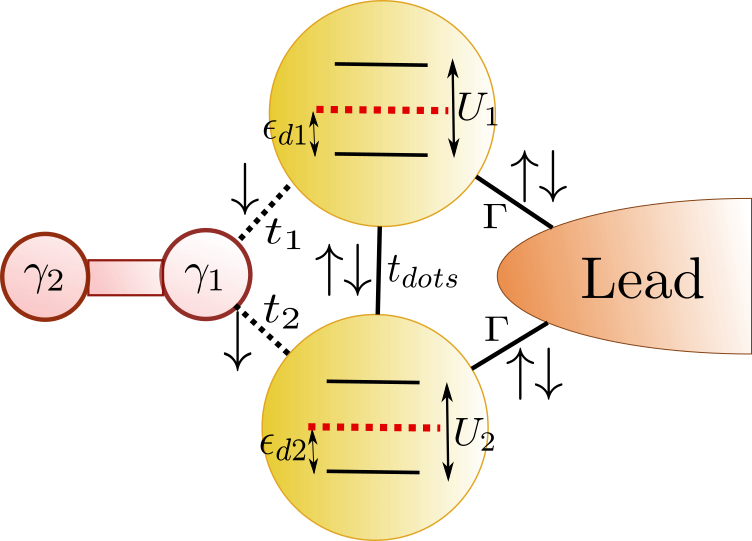
\includegraphics[scale=0.4]{Graficos/Model.png}
\caption{ DQD-Majorana set-up. Solid lines represent standard coupling interactions. Dashed lines represent majorana spin-$\dw$ effective couplings \eqref{eq:Majorana-ham}. The atomic-limit energy levels are plotted inside each QD. $\ed{i}$ is the particle's energy inside QD$i$ and $U_i$ is the corresponding coulomb potential. The red dashed lines represent the Fermi level.  
}
%
\label{fig:GenModel}
\end{center}
\end{figure}
%-----------E N D  F I G U R E  1 ------


For the DQD-lead system, we can implement the Anderson Model so that 
%d_{i\sigma}^{\dagger}d_{i\sigma}
\begin{align*}
H_{DQD}=& \sum_{\sigma} \sum_{i\in\{1,2\}}\left(\epsilon_{di}+\frac{U_i}{2}\right)\hat{n}_{i\sigma}+ \frac{U_i}{2}(\sum_{\sigma} \hat{n}_{i\sigma}-1)^{2} \\
&\ \ \ \ \ + \sum_{\sigma \in \{\up , \dw\}} \tdots(\dann_{1\sigma}  d_{2\sigma}+\dann_{2\sigma}  d_{1\sigma}),
\end{align*}
%
where $\ed{i}$ represents the energy level of each QD, $U_i$ is the Coulomb repulsion and $\tdots$ is the coupling between both QDs. In addition the operator $\dann_{i\sigma}$ creates a particle in dot $i$ with spin $\sigma$ and $\hat{n}_{i\sigma}:=d_{i\sigma}^{\dagger}d_{i\sigma}$ is the particle number operator of this state. On the other hand, the interaction with the Lead is described by 

\LUIS{Pls add a ``label'' to EVERY equation and EVERY figure.}

\begin{eqnarray*}
H_{Lead} & = & \sum_{\mathbf{k}\sigma }\epsilon_{\mathbf{k}}c_{\mathbf{k}\sigma }^{\dagger}c_{\mathbf{k}\sigma }\\
H_{DQD-Lead} & = &  \sum_{\mathbf{k}\sigma }\sum_{i\in\{1,2\}}\Gamma_i c_{\mathbf{k}\sigma }^{\dagger}d_{i\sigma}+\Gamma_i d_{i\sigma}^{\dagger}c_{\mathbf{k}\sigma },
\end{eqnarray*}
%
where the sum over $\mathbf{k}$ is performed over all possible crystal momentums in the lead. The operator $c_{\mathbf{k}\sigma }^{\dagger}$ creates a particle with momentum $\mathbf{k}$ and spin
$\sigma$ in the lead, $\epsilon_{\mathbf{k}l}$ is the energy
of the lead's particles and $\Gamma_i$ is the hopping exchange
term between the lead each $QD$ . \\

To model the interaction between the DQD and the Majorana Mode we define the majorana operators as the  superposition of the creation and annihilation operators of a spin $\dw$ particle $f_\dw$:

$$\gamma_1 := \frac{1}{\sqrt{2}} \left( f^\dagger_{\dw} + f_{\dw}\ \right) , \gamma_2 := \frac{1}{\sqrt{2}} \left( f^\dagger_{\dw} - f_{\dw} \right).$$
This makes possible to define an effective coupling between the Majorana Mode and the DQD by attaching $\gamma_1$ with the spin-$\dw$ channel in the QDs

%H_{TS} & = & 2\epsilon_{m}\gamma_{1}\gamma_{2}\nonumber \\
\begin{eqnarray}
H_{M-DQD} & = &  \sum_{i}t_{i} \left(d_{i\downarrow}^{\dagger}\gamma_{1}+\gamma_{1}d_{i\downarrow}\right) \\
& = &  \sum_{i}t_{i} \left(d_{i\downarrow}^{\dagger}f^\dagger_{\dw} + 
f_{\downarrow}d_{i\dw} +d_{i\downarrow}^{\dagger}f_{\dw}+
+f_{\downarrow}^{\dagger} d_{i\downarrow}\right).
\label{eq:Majorana-ham}
\end{eqnarray}


\Jesus{Should I put the other terms? }


This effective coupling represents the single majorana mode at the edge of the TS attached to the QD. \citeauthor{ruiz-tijerina_interaction_2015}  proved that the interaction \eqref{eq:Majorana-ham} is able to reproduce effectively the results obtained when the Kitaev chain in the topological phase is attached to a single QD.  \\
 

\subsection{Methods}
In order to calculate the properties of the model given by Eq.\ (\ref{eq:Majorana-ham}), we used the Numerical Renormalization Group (NRG) approach. \cite{wilson_renormalization_1975,sindel_numerical_2005,bulla_numerical_2008} 
 To to improve the efficiency of the code we used the symmetries of the system.  Now, one of the insights of this model is that spin-$\dw$ particle number $\hat{N_\dw}$ is not preserved due to the term $(d_{i\downarrow}^{\dagger}f^\dagger_{\dw} + 
f_{\downarrow}d_{i\dw})$ in $H_{M-DQD}$ \eqref{eq:Majorana-ham}. However the  spin-$\up$ particle number $\hat{N}_\up$ and the parity of spin-$\dw$ particles $\hat{P}_\dw = \pm $ ($+$ even, $-$ odd) are still conserved. \\

To implement the NRG code it is necessary to define a cut-off energy $D$ \cite{bulla_numerical_2008}. By convention, we define this energy to be double the coulomb repulsion of the first dot $D = 2U_1$. For convenience we use $D$ as energy unit.  \\


The local density of states (LDOS) on each dot is obtained by computing the spectral function 

\begin{equation}
    \rho_{i\sigma}(\omega)= \frac{-i}{\pi}\mathcal{I}\left[ \mathcal{G}^R_{i\sigma}(\omega) \right],
    \label{eq:SpectralFunction}
\end{equation}
%
where $\mathcal{G}^R(\omega)$ is the Fourier transform of the Green function $\mathcal{G}^R(t,T)=-i\theta(t) \langle \{d_{i,\sigma}(t) , d_{i,\sigma}^\dagger(0)\} \rangle$. The spectral functions were calculated with the DM-NRG method.\cite{hofstetter_generalized_2000} 



\Jesus{Luis... should I put details about the methods that we used?. Till now, I just mentioned them with references. }
\LUIS{It is fine for now}
%(NRG) method [44–46]: one can refer Ref. 47 for a review.
%For better efficiency, we exploit the symmetries that our sys-
%tem has: [Q ↑ , H] = [P ↓ , H] = 0 where Q ↑ and P ↓ are
%charge number operator for spin-↑ electrons and parity op-
%erator for the sum Q ↓ of spin-↓ electrons and f electrons, re-
%spectively. Note that the QD-MFS hopping changes Q ↓ by
%even numbers only. For the
%we calculate the spec-where |ni is
%the many-body eigenstate with energy E n and |0i is th






\subsection{Atomic limit}
\label{sec:AtomicLimit}


In the atomic limit $(\Gamma = 0)$ the lead interaction is neglected. Hence the Hamiltonian \eqref{eq:Ham} reduces to 

    \begin{equation}
        H=H_{DQD}+H_{M-DQDs}.
    \end{equation}
    
The dimension of this Hamiltonian is $2^2\times2^2\times 2 =32$ ($2^2$ per QD $\up$, $\dw$ and $2$ due to the majorana spin-$\dw$). 

A simple analytical solution can be given for the case where  $\ed{i}=\frac{-U_i}{2}=\frac{-U}{2}$ and $\tdots = 0$. With

    \begin{eqnarray}
        H=  & \frac{U}{2}\sum_i(\sum_{\sigma} \hat{n}_{i\sigma}-1)^{2} +  \sum_{i} t_i \left(d_{i\downarrow}^{\dagger}\gamma_{1}+\gamma_{1}d_{i\downarrow}\right).
        \label{eq:AtomicHam}
    \end{eqnarray}

    % \begin{eqnarray}
    %     H=  & \frac{U}{2}\sum_i(\sum_{\sigma} \hat{n}_{i\sigma}-1)^{2} + t \sum_{i} \left(d_{i\downarrow}^{\dagger}\gamma_{1}+\gamma_{1}d_{i\downarrow}\right).
    %     \label{eq:AtomicHam}
    % \end{eqnarray}

Hamiltonian \eqref{eq:AtomicHam} can be written in blocks labeled by the  two conserved quantum numbers $\hat{N}_\up $ and $\hat{P}_\dw = \pm$ . For example the block  for $0$ spin-$\up$  and odd spin-$\dw$ particles  $\left( \hat{N}_\up =0, \hat{P}_\dw = - \right)$ can be written in terms of the base 
    \begin{equation}
        \lbrace \ket{\dw,\dw,\dw} , \ket{0,0,\dw} , \ket{0,\dw,0}, \ket{\dw,0,0}     \rbrace;
    \end{equation}
where the states are labeled by  $\ket{QD1,QD2,MZM}$. Hence the representation of block $\left( \hat{N}_\up =0, \hat{P}_\dw = - \right) $ is 
    \begin{equation}
    \begin{array}{c}
        \vert\downarrow,\downarrow,\downarrow\rangle\rightarrow\\
        \vert0,0,\downarrow\rangle\rightarrow\\
        \vert0,\downarrow,0\rangle\rightarrow\\
        \vert\downarrow,0,0\rangle\rightarrow
        \end{array}\left[\begin{array}{cccc}
        0 & 0 & -t_1 & t_2\\
        0 & U & t_2 & t_1\\
        -t_1 & t_2 & \frac{U}{2} & 0\\
        t_2 & t_1 & 0 & \frac{U}{2}
    \end{array}\right].
    \end{equation}

The four eigen-energies of this block of the Hamiltonian can be written as \LUIS{Let's call these energy states something!}
%
    \begin{eqnarray}
        \varepsilon^{(1)}_{\pm} = & U/4 \pm  \sqrt{\frac{U^2}{16} + t_1^2+t_2^2} \\ \nonumber 
        \varepsilon^{(2)}_{\pm} = &  \frac{3U}{4} \pm  \sqrt{\frac{U^2}{16}+ t_1^2+t_2^2} \; .
        \label{eq:atomiclimit1}
    \end{eqnarray}
    % \begin{equation}
    %     U/4 \pm  \sqrt{\frac{U^2}{16} + 2t^2} \ , \ 3U/4 \pm  \sqrt{\frac{U^2}{16}+ 2t^2}.
    % \end{equation}
For $t << \frac{U}{4}$, the eigenvalues can be approximated by the Taylor series giving
    \begin{eqnarray}
        \varepsilon^{(1)}_{\pm} \approx & U/4 \pm  U/4 \left(1 + 8\frac{t_1^2+t_2^2}{U^2} \right) \\ \nonumber
        \varepsilon^{(2)}_{\pm} \approx &  \frac{3U}{4} \pm  U/4 \left(1 + 8\frac{t_1^2+t_2^2}{U^2} \right) \; .
        \label{eq:atomiclimit2}
    \end{eqnarray} 
    % \begin{equation}
    %     U/4 \pm  U/4 \left(1 + \frac{16t^2}{U^2} \right)+  \ , \ 3U/4 \pm  U/4 \left(1 + \frac{16t^2}{U^2} \right).
    % \end{equation}

Comparing this results with the $t=0$ eigen-values $(0,\frac{U}{2},U)$, we observe that the displacement of the energy levels  generated by the majorana couplings $t_1$ and $t_2$ is 

    \begin{equation}
        \delta_{t_1,t_2} = \frac{2t_1^2+2t_2^2}{U}.
        \label{eq:displacement}
    \end{equation}

This implies that the energy scale where the majorana effects will be observed will scale as the square root of the energy couplings. A similar result will be obtained for the other quantum numbers. 


\Jesus{The analysis that I did explains the energy scale where the majorana peaks appear. But I don't know if it is good to do the base change that is the way we used to explain the Kondo satellites. }

\LUIS{No need to change the basis. But can you add some dashed lines in the plots of Fig. 3 showing these values as a reference? }

% It is now suitable to do change to the basis of symmetric ($d_+$) and anti-symmetric ($d_-$) states 
% \[
%   d_{+ , \sigma} = \frac{1}{\sqrt{2}} (d_{1\sigma} +d_{2\sigma}) \ , \ 
%   d_{- , \sigma} = \frac{1}{\sqrt{2}} (d_{1\sigma} -d_{2\sigma}),
% \]



% where Hamiltonian \eqref{eq:AtomicHam}  looks like 
% \begin{align}
% H = \sum_{\sigma}  \frac{U}{4}\left( \left( \hat{N}-2 \right)^2- \hat{E}^2 \right) + \frac{t}{\sqrt{2}} (\gamma_1 d_{+,\dw}+d^\dagger_{+,\dw}\gamma_1 ).
% \label{eq:ExchangeHam}
% \end{align}


% where  $\hat{N} = \sum_\sigma (\hat{n}_{+,\sigma} + \hat{n}_{-,\sigma})$ is the total particle number and $\hat{E} = \sum_\sigma (d^\dagger_{+,\sigma}d_{-,\sigma} + d^\dagger_{-,\sigma}d_{+,\sigma})$ is a term representing the state exchange between $+$ and $-$ spaces. An schematic representation of this interaction is observed in Figure \ref{fig:ExchangeModel}.



% %-----------F I G U R E  2 ------
% \begin{figure}[tb]
% \begin{center}
% 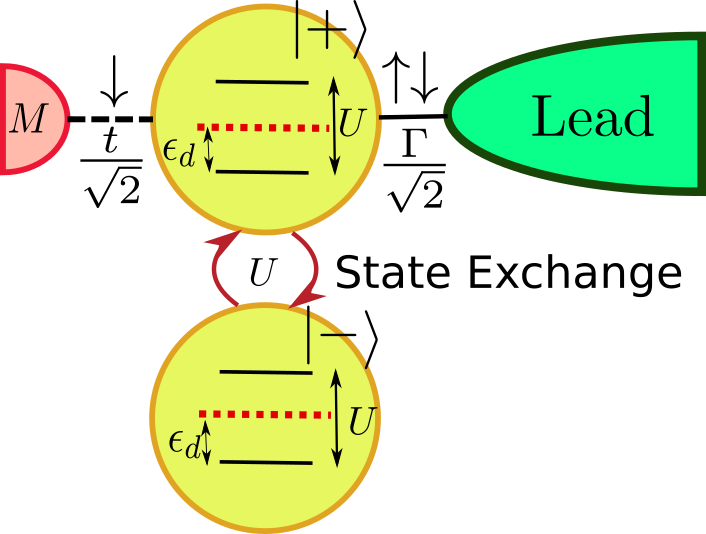
\includegraphics[scale=0.35]{Graficos/ExchangeMod.png}
% \caption{ Schematic representation of Hamiltonian \eqref{eq:ExchangeHam} After the base-change, only the symmetric state $ d^\dagger_+$ is coupled to Majorana mode. The majorana coupling is cut to $\frac{t}{2}$ and there appears an exchange term between the symmetric and the $ d^\dagger_+$ and the $ d^\dagger_-$ anti-symmetric state. 
% }
% %
% \label{fig:ExchangeModel}
% \end{center}
% \end{figure}
% %-----------E N D  F I G U R E  2 ------








%Using the symmetries of the system , $\hat{N}_\up$ and $P_\dw$ conservation, we can divide it into blocks of size $4\times4$. 




\section{NRG Results}
\label{sec:Results}

%---------------------t1=t2----------------------------------------------

\subsection{Connecting the Majorana Mode \label{sub:t1=t2}}

\textbf{Parameters:}

    $\Gamma \sim 2.83\times10^{-2}D,\  t_{dots}=0 ,\  U_{1,2} = -2\ed{1,2} = 0.5D.$

\textbf{Variable:}
    $$t_1=t_2 \in [0\  ,\  2\times10^{-2}D].$$
%----------------------FIGURE 2--------------------------------
    \begin{figure}[bt]
    \centering
    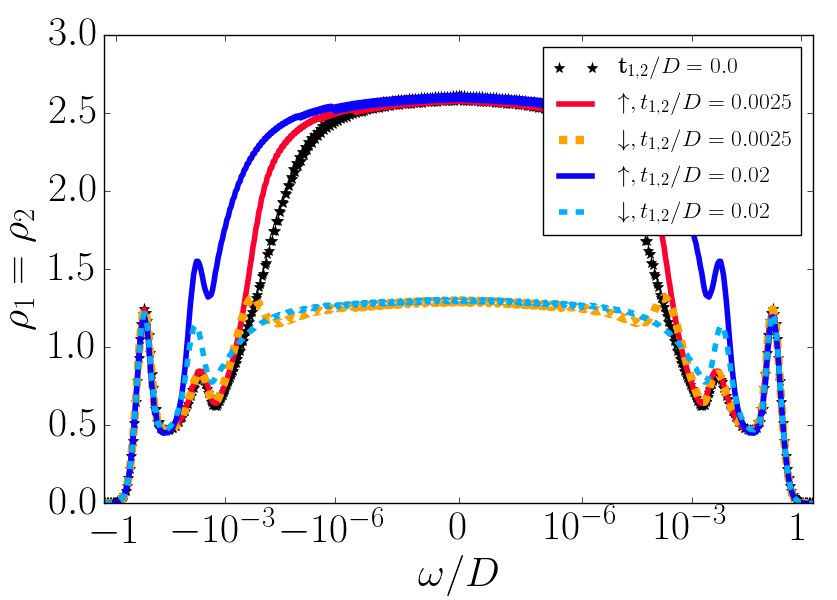
\includegraphics[scale=0.35]{Graficos/LogPlot.png}
    \caption{\label{fig:t1=t2/logplot} Density of states at each QD of the horizontal dashed cuts in Figure \ref{fig:t1=t2-2D} . The energy is in logarithmic scale. At the Fermi energy $(\omega =0)$ the spin-$\up$ DOS is $\rho_\up(0) \sim \frac{1}{4\pi\Gamma}$. At $t_{1,2}=0$ $\rho_up=\rho_\dw$. However, for  $t>0$  $\rho_\dw(0) = \frac{\rho_\up(0)}{2}$ which is a majorana signature. The spin-$\up$ and spin-$\dw$ DOS split at an energy scale that depends on the parameter $t_{1}=t_2$.}
    \end{figure}
%------------------------------------------------------


    
The first process consists in attaching the Majorana mode to both Quantum Dots symmetrically. For this, we scale up the coupling parameter $t_1=t_2$ from $0D$ (Decoupled) to $0.02D$ (Completely coupled). The other parameters where chosen with an equilibrium between the dot energy and Coulomb repulsion $(\ed{1,2}=-\frac{U_{1,2}}{2})$  and  without inter-dot coupling $t_{dots}=0$. These circumstances guarantee that the system preserves Particle Hole Symmetry (PHS). Thus the Density of States (DOS) of particles and holes remains equal at all instances $(\rho(-\omega) = \rho(\omega))$. \\
    
For $t_1 =t_2 = 0$ the system consists only of a DQD coupled to a NM lead. Since the model is symmetric for both QDs , the Kondo density of states  splits between both dots (See Figure \ref{fig:t1=t2/logplot}). Apart from the coulomb peaks that appear at $\omega=0.25D=\pm \ed{1,2}$, two new sided peaks emerge at low-energies $(\omega \sim 10^{-2}D)$. These peaks are the result of the of a strong anti-ferromagnetic interaction between both dots caused by the indirect exchange of quantum states through the Lead. This interaction receives the name of Ruderman-Kittel-Kasuya-Yosida (RKKY) interaction\cite{ruderman_indirect_1954,kasuya_theory_1956,yosida_magnetic_1957}. \\
    
    

Once the MZM is attached $t_1 =t_2 > 0$ the spin-$\up$ and spin-$\dw$ DOS split at low energies. In both dots the spin-$\dw$ DOS at the Fermi energy ($\omega =0$) decays to the half of the spin-$\up$ DOS $\rho_\dw = \frac{\rho_\up}{2} $. It was previously verified  by  \citeauthor{ruiz-tijerina_interaction_2015} that the Majorana signature of a QD in the Kondo regime coupled to a TS wire is the half-decay of the spin-$\dw$ DOS. Hence the results from Figure \ref{fig:t1=t2/logplot} imply that the majorana signature appears in both dots. \\
    
Moreover, there is an additional effect caused by the indirect exchange between the QDs through the Majorana mode. The energy scale of this effect was computed for the atomic limit in equation \eqref{displacement}. Depending on this energy scale the consequences the indirect exchange through the majorana mode will produce different results.

%The consequences of this effect depend on the energy range of the majorana couplings $t_1=t_2$.
    
\begin{enumerate}
    \item If $t_1=t_2 \ll \Gamma $ two more satellites are formed at very low energies only in the spin-$\dw$ DOS. These peaks correspond to the displacement energy $\frac{4t^2}{U}$ found in the atomic limit \eqref{displacement}  (See Figure \ref{fig:t1=t2-2D} Spin-down $\omega \sim 10^{-3}D$ ). 
    \item For $t_1=t_2 \sim \Gamma$ the Majorana peaks do not appear in the spin-$\dw$ DOS any more. Instead, we observe a combined Kondo-majorana physics in the satellite peaks. This produces an increase of the DOS at the energy scale where the satellite peaks appeared at $t_1=t_2=0$. Since $\rho_\up$ must double $\rho_\dw$ at $\omega=0$, the spin-$\up$ satellites are greater (See  \ref{fig:t1=t2/logplot} for $t_{1,2}=0.02D$). This effect causes the rapid scale-up of satellite peaks for $t_1=t_2>0.01D$  (See \ref{fig:t1=t2-2D} Spin-$\up$, $\omega \sim 10^{-2}D$).
    
\end{enumerate}
    
    \Jesus{Maybe we should include a plot comparing the temperature of Kondo and majorana physics.}

    \begin{figure}[bt]
        \begin{center}
            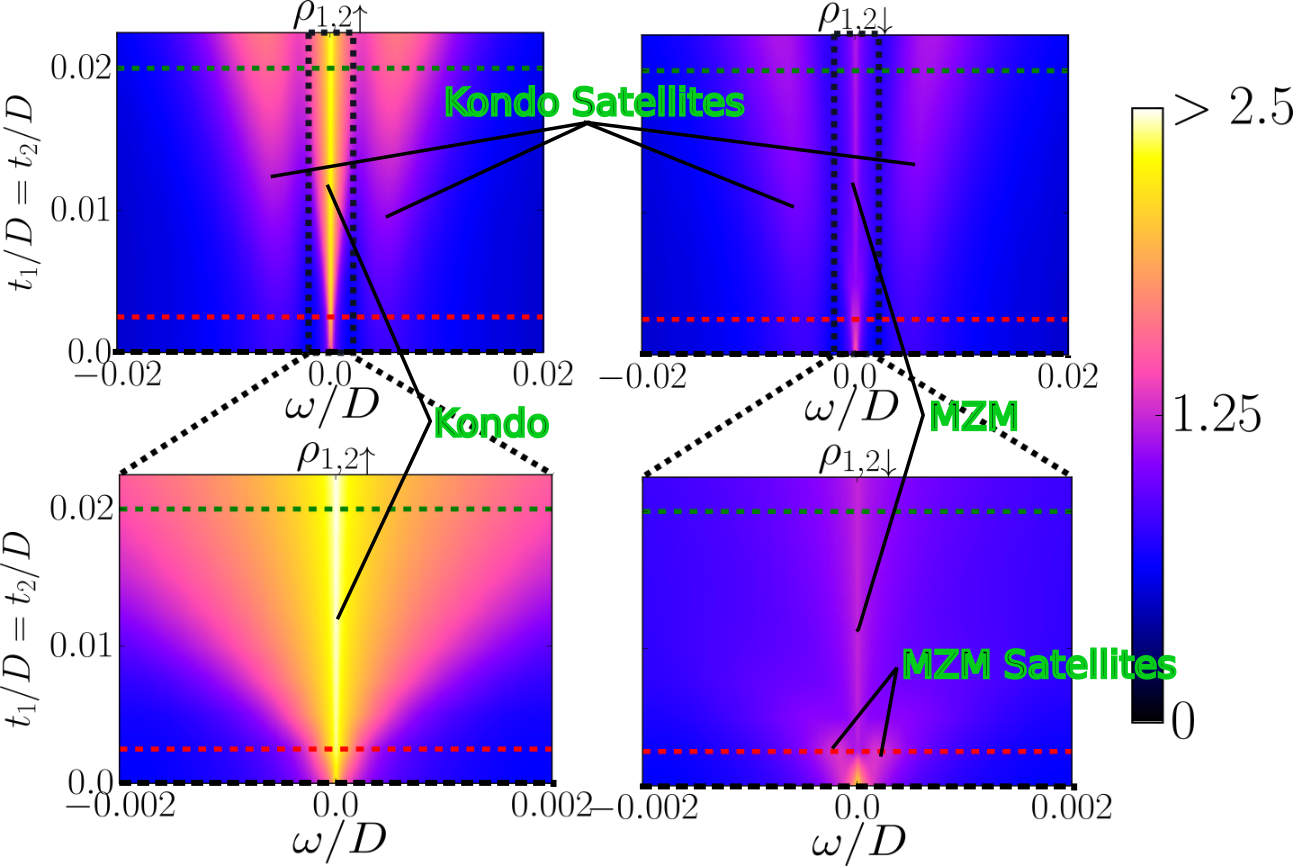
\includegraphics[scale=0.26]{Graficos/t1=t2-2D.png}
            \caption{\label{fig:t1=t2-2D}Evolution of the DOS of both QDs through $t_1 = t_2$ tuning. UP: Energy scale $\omega \sim 10^{-2}D$. DOWN: Energy scale $\omega \sim 10^{-3}D$. LEFT: Spin $\up$. RIGHT: Spin $\dw$. \LUIS{IN the paper plot you need to remove to comments ``MZM satellites'', etc. We can add small arrows and explain in the main text.}}
            \end{center}
    \end{figure}
    
%-----------------------------e2------------------------------------------    
\subsection{Transferring the MZM \label{sec:e2}}

\textbf{Parameters:}

\begin{align*}
    \Gamma \sim 2.83*10^{-2}D, t_{dots}= & 0 , U_{1,2} = -2\ed{1} = 0.5 \\
    t_1=t_2=&0.02D
\end{align*}
\textbf{Variable:}
$$\ed{2} \in [-0.25D \  , -0.05D]$$

This process starts in the final state of \ref{sub:t1=t2} with the DQD coupled symmetrically to the Majorana mode and $t_1=t_2=0.02D$. The idea of this process is to break PHS by increasing the energy of the second QD $\ed{2}$. This procedure should induce the Majorana to tunnel only into the first dot. \\


\begin{figure}[bt]
\centering
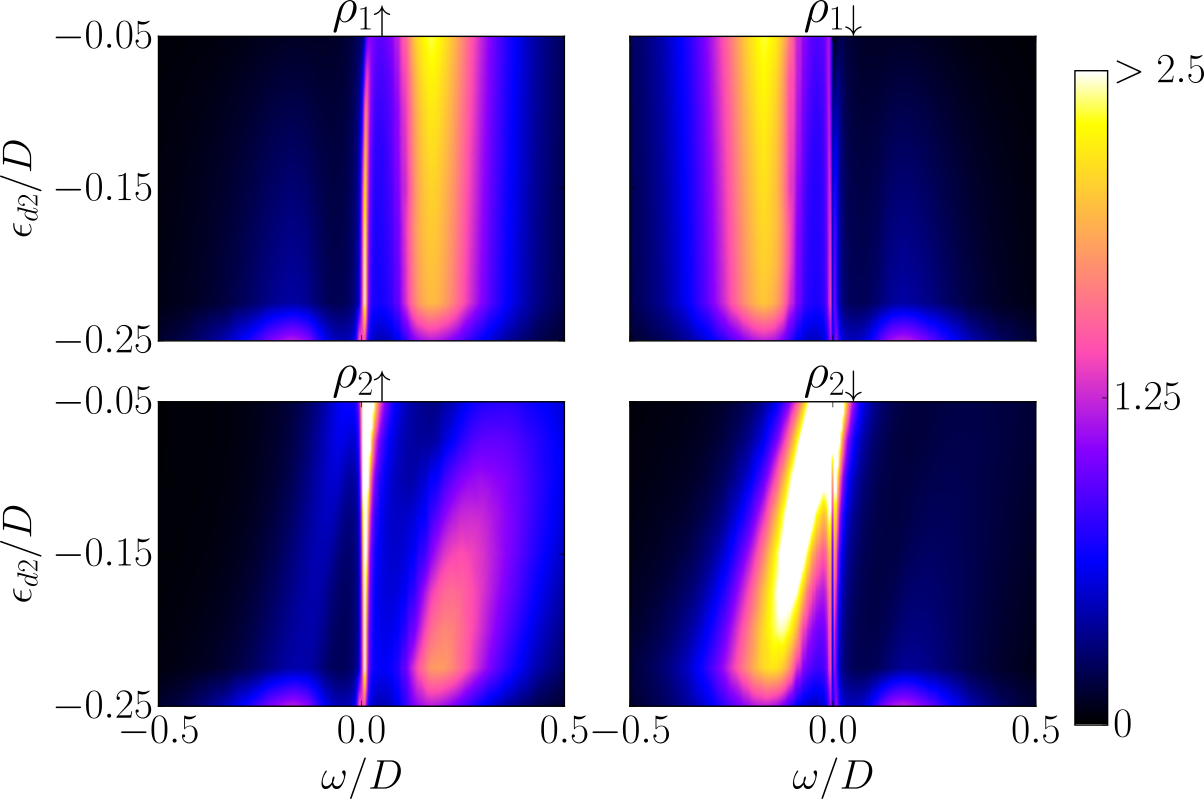
\includegraphics[scale=0.3]{Graficos/2Dhigh.png}
\caption{\label{fig:2D/Shift_ed2} Evolution of the DOS of both QDs through the $\ed{2}$ tuning. UP: QD1. DOWN: QD2. LEFT: Spin $\up$. RIGHT: Spin $\dw$.}
\end{figure}


In \ref{fig:2D/Shift_ed2} we observe that both, the Kondo and the MZM peaks are preserved in the first QD as well as the majorana signature (See \ref{fig:ed2/Fermi}) when $\ed{2}$ is scaled up to $-0.1$.  However,  PHS breaking will favor the growth of the spin-$\up$ hole $(w>0)$  satellite and the spin-$\dw$ particle $(w<0)$ satellite.


\begin{figure}[bt]
\centering
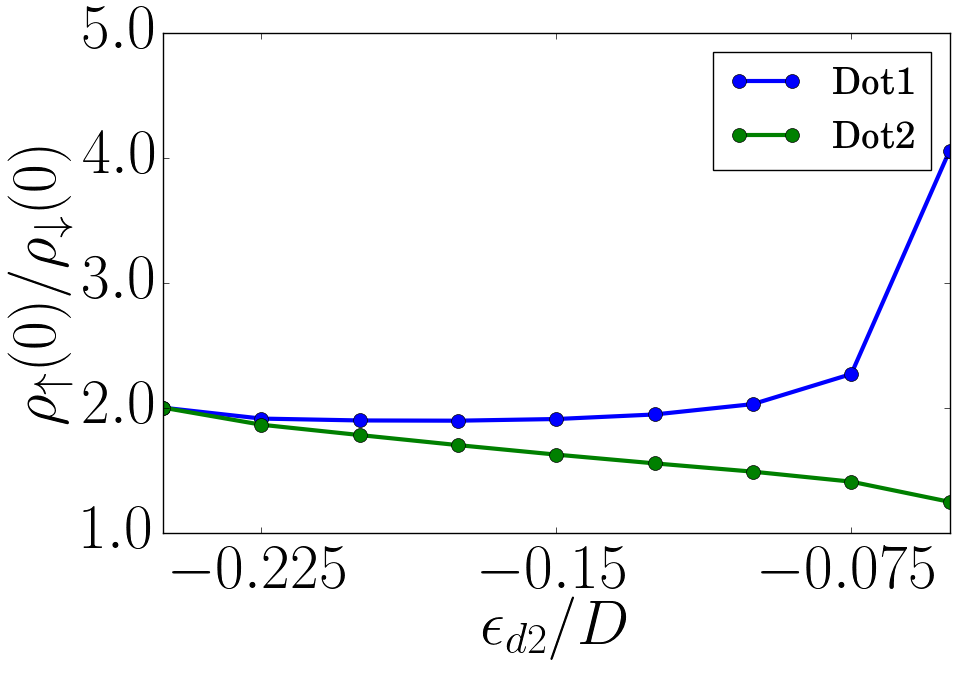
\includegraphics[scale=0.3]{Graficos/e2-Fermi.png}
\caption{\label{fig:ed2/Fermi} As described in \ref{sub:t1=t2} the relation $\frac{\rho_\up(0)}{\rho_\up(0)}=2$ determines the Majorana Signature . This picture shows the evolution of the relation $\frac{\rho_\up(0)}{\rho_\up(0)}$ for both QDs. While QD2 losses rapidly the Majorana signature, QD1 maintains it till $\ed{2}\sim -0.1D$. For  $\ed{2}>-0.1D$ the coulomb peaks in QD2 overlap with the fermi energy which destroys the Kondo effect in the first dot (See Figure \ref{fig:2D/Shift_ed2}). }

\end{figure}



%---------------------------------------------------------------------------

%---------------------------------------------------------------------------





    
\section{Concluding remarks}
\label{sec:Conclusions}

Conclusion goes here.

\begin{acknowledgments}
The authors thank Edson Vernek for enlightening discussions.  L.G.G.V.D.S. acknowledges financial support by CNPq (grants No. 307107/2013-2 and 449148/2014-9), and FAPESP (grant No. 2016/18495-4).
\end{acknowledgments}

\LUIS{Only ONE bib file}

%---------------------- Apendix A------------------------


%-----------------------------------------------------------

%\bibliographystyle{unsrtnat}
%\addcontentsline{toc}{section}{\textbf{References}}
\bibliography{Majorana_DQD}




\end{document}


% \appendix

% \section{Atomic limit: Change of basis}
% Returning to Hamiltonian \eqref{eq:AtomicHam} the change of basis is given by 
% \[
%   d_{+ , \sigma} = \frac{1}{\sqrt{2}} (d_{1\sigma} +d_{2\sigma}) \ , \ 
%   d_{- , \sigma} = \frac{1}{\sqrt{2}} (d_{1\sigma} -d_{2\sigma}).
% \]

% These new operators satisfy the fermionic anti-commutation relations 
%  \[ \{d_{\pm , \sigma}, d^\dagger_{\pm , \sigma}\} = 1 , \{ d_{\pm , \sigma}, d^\dagger_{\mp , \sigma}\} = 0,
% \]
%  so that the may be considered as fermion operators. All lineal terms in \eqref{eq:AtomicHam} are trivially adapted to the new base. The repulsion potential 
% $$\sum_{i} (\sum_{\sigma} d_{i \sigma}^{\dagger}d_{i \sigma}-1)^{2} = (\sum_{\sigma} d_{1 \sigma}^{\dagger}d_{1 \sigma}-1)^{2} + (\sum_{\sigma} d_{2 \sigma}^{\dagger}d_{2 \sigma}-1)^{2} . $$ 
% gives rise to a non-trivial interaction between the new states. To find this interaction we define the particle number operator  
% \[\hat{n}_{i,\sigma}:= d^\dagger_{i,\sigma}d_{i,\sigma}.\] 

% So that 
% \begin{align}
% \hat{n}_{1,\sigma}= & \frac{1}{2} \left( \hat{n}_{+,\sigma} + \hat{n}_{-,\sigma} + d^\dagger_{+,\sigma}d_{-,\sigma} + d^\dagger_{-,\sigma}d_{+,\sigma} \right) \\
% = & \frac{1}{2} \left( \hat{N}_\sigma + \hat{E}_\sigma \right),
% \end{align}
% with $\hat{N}_\sigma = \hat{n}_{+,\sigma} + \hat{n}_{-,\sigma}$ and $\hat{E}_\sigma = d^\dagger_{+,\sigma}d_{-,\sigma} + d^\dagger_{-,\sigma}d_{+,\sigma}. $ Similarly 

% \[\hat{n}_{2,\sigma}= \frac{1}{2} \left( \hat{N}_\sigma - \hat{E}_\sigma \right).  \]
% Hence 
% \begin{align}
% \sum_{i} (\sum_{\sigma} d_{i \sigma}^{\dagger}d_{i \sigma}-1)^{2} = & \left(\frac{\hat{N} +\hat{E}}{2}-1 \right) ^{2} + \left( \frac{\hat{N} -\hat{E}}{2}-1 \right)^{2} \\
%  = & \frac{\left( \hat{N}-2 \right)^2- \hat{E}^2}{2},
% \end{align}

% with $\hat{N}_\sigma=\sum_\sigma \hat{N}_\sigma $ , $\hat{E}=\sum_\sigma \hat{E}_\sigma $. Note that opeator $\hat{N}$ represents the total occupation number inside both dots. If this occupation is different than $2$ there is an imbalance between particles and dots that is punished by this term. The term $E^2$ is much more interesting since this one is the responsible for the emergence of satellite peaks in the DOS. To understand what it makes it is simple to observe its results when applied to a based ordered by $\vert + , - \rangle$. 
% \[ \hat{E}^2 \vert \up , 0 \rangle =  \hat{E} \vert 0 , \up \rangle = \vert \up , 0 \rangle   \] 
% \[ \hat{E}^2 \vert \up , \dw \rangle =  \hat{E} \left( \vert 0 , \up\!\dw \rangle + \vert \up\!\dw , 0 \rangle \right) = 2\vert \up , \dw \rangle - 2\vert \dw , \up \rangle  \]

% \begin{align}
% H = \sum_{\sigma}  \frac{U}{4}\left( \left( \hat{N}-2 \right)^2- \hat{E}^2 \right) + \frac{t}{\sqrt{2}} (\gamma_1 d_{+,\dw}+d^\dagger_{+,\dw}\gamma_1 )
% \label{t+}
% \end{align}